%!TeX program = xelatex
\documentclass[12pt,hyperref,a4paper,UTF8]{ctexart}
\usepackage{BNUpapers}

%%-------------------------------正文开始---------------------------%%
\begin{document}
\begin{sloppypar}

%%-----------------------封面--------------------%%
\cover

%%------------------摘要-------------%%
%\begin{abstract}
%
%在此填写摘要内容
%
%\end{abstract}

\thispagestyle{empty} % 首页不显示页码

%%--------------------------目录页------------------------%%
\newpage
\tableofcontents

%%------------------------正文页从这里开始-------------------%
\newpage

%%可选择这里也放一个标题
%\begin{center}
%    \title{ \Huge \textbf{{标题}}}
%\end{center}

\section{智慧公路建设的必要性和意义}

近年来,以物联网与人工智能技术的智慧公路建设成果了国家发展的重点工程之一。国家 “新基建”“数字中国” 等战略部署明确要求发展智慧公路,《交通强国建设纲要》将其列为重要任务。智慧公路建设是积极应对当前公路网在交通安全、运行效率、服务水平、管理能力等方面面临诸多挑战,实现我国公路交通高质量发展的有效途径。我国公路网规模虽居世界首位,但面临道路安全事故频发、智能化信息服务水平不高、绿色发展压力大等问题,而积极高效建设智慧公路是解决上述问题和矛盾、构建智慧交通体系、践行交通强国战略的主要途径。从智能交通技术发展看,以人工智能、5G等数字化技术主导的新一轮科技革命和产业变革风起潮涌,科技创新为交通运输高质量发展带来广阔空间,积极发展智慧公路成为公路交通高质量发展的必由之路。

智慧公路建设意义重大。它能提升道路安全保障、运行效率、服务管理和绿色发展水平。通过综合运用多种信息技术和工程技术,构建全域感知、泛在互联等能力,实现建设、运营、养护、服务全寿命期智慧化,可有效应对公路发展中的安全、效率等目标要求。其功能特征包括全域感知、泛在互联、融合计算等,能实现多要素信息获取、不同领域信息互联、多类型数据处理等,为各类型用户提供服务。从发展现状看,各地开展智慧公路建设试点示范,推进信息技术与高速公路深度融合,验证了智慧赋能的有效性。长远来看,智慧公路建设分近期、中期、远期阶段,通过实现各阶段目标,可全面建成智慧公路网络体系,提升关键技术自主可控能力,使智慧化能力覆盖全要素、全场景等,进入国际前列,达到世界领先水平,在构建综合运输体系、保障国家发展安全中发挥关键作用,驱动公路行业可持续发展,支持实现交通强国建设。在重点任务方面,涵盖智慧化建造、基础设施数字化、车路协同自动驾驶等,这些任务的落实将进一步推动智慧公路发展,发挥其在安全、效率、服务等多方面的价值。相关研究成果突出系统性、前瞻性、可实施性,以期促进智慧公路健康发展、深化智慧公路技术探索与应用实践。

\begin{figure}[!htbp]
    \centering
    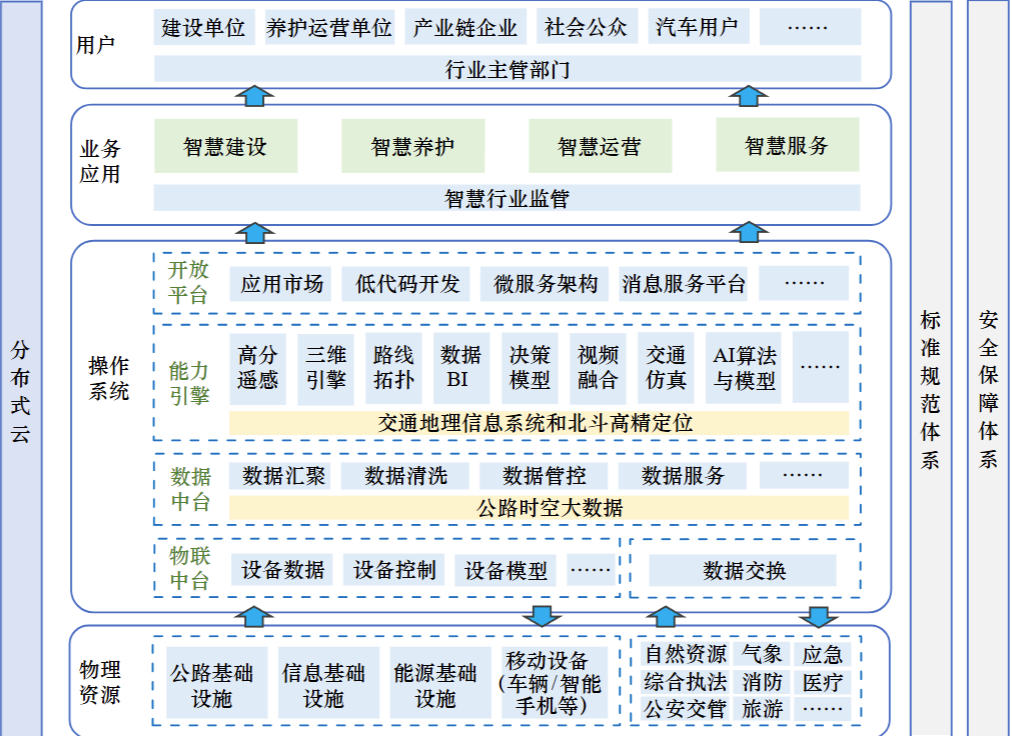
\includegraphics[width =.6\textwidth]{figures/智慧公路总体架构.png}
    \caption{智慧公路总体架构}
    \label{framework}
\end{figure}

当前公路网发展面临诸多核心问题,包括道路安全事故频发,气候和欠养护导致限制通行时有发生,智能化信息服务水平不高、用户出行体验欠佳,道路交通在交通全行业中碳排放占比较高、绿色发展压力较大,且存在对智慧公路内涵理解差异大、缺乏统一认识和整体规划,标准规范体系不健全,支持发展的创新性政策规章缺失,跨部门协同治理机制尚未理顺等问题。发展智慧交通可通过综合运用大数据、云计算、物联网、AI 等信息技术及智能装备、新材料、新能源等工程技术,构建全域感知能力以整合多种信息采集手段获取多要素实时信息,实现泛在互联以打通公路与公路、路域环境及其他 “三网” 的信息互联,借助融合计算与分析决策能力对多类型数据处理并支持智慧分析和决策,通过智能协同实现公路各环节及跨区域业务协同,利用服务触达能力提供实时便捷的出行服务,从而提升道路安全保障、运行效率、服务管理及绿色发展水平,解决公路网现存的安全、效率、服务、管理等核心问题。




\reference

\end{sloppypar}

\end{document}